\documentclass[11pt, oneside]{article}   	% use "amsart" instead of "article" for AMSLaTeX format
\usepackage{geometry}                		% See geometry.pdf to learn the layout options. There are lots.
\geometry{letterpaper}                   		% ... or a4paper or a5paper or ... 
%\geometry{landscape}                		% Activate for for rotated page geometry
%\usepackage[parfill]{parskip}    		% Activate to begin paragraphs with an empty line rather than an indent
\usepackage{graphicx}				% Use pdf, png, jpg, or eps� with pdflatex; use eps in DVI mode
								% TeX will automatically convert eps --> pdf in pdflatex		
\usepackage{amssymb}
\usepackage{amsmath}
\usepackage{parskip}
\usepackage{color}

\title{Kepler (from Varberg text)}
%\author{The Author}
%\section{}
% \subsection*{R code}
\date{}							% Activate to display a given date or no date

\graphicspath{{/Users/telliott_admin/Dropbox/Tex/png/}}

% \begin{center} 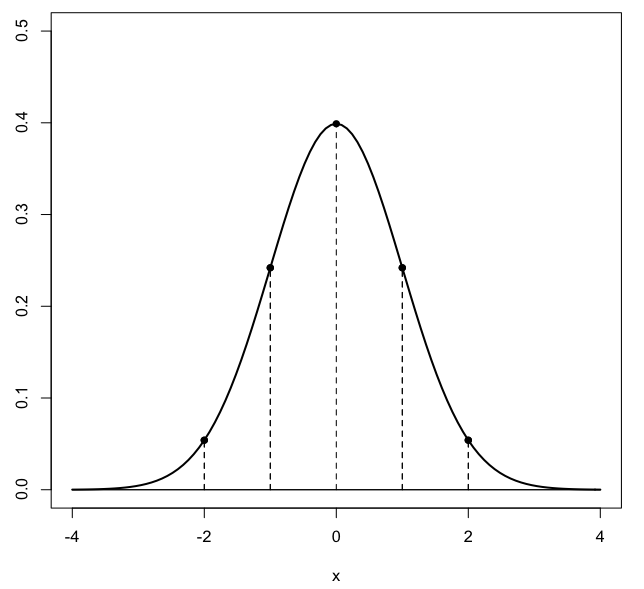
\includegraphics [scale=0.4] {gauss3.png} \end{center}

\begin{document}
\maketitle
\Large
\noindent

This short write-up is my attempt to work through the derivation of Kepler's three laws in the text Varberg \emph{Calculus} (online version only, Chapter 14).  One change I feel I need to introduce is to use $\mathbf{r}$ for the position vector (following Feynman) rather than $\mathbf{X}$, as Varberg do.

\subsection*{Example 14.4}

Before starting on the proofs, we have two preliminary examples to work through that give results we will use later.  The first one introduces $\mathbf{L}$, described as a unit vector-valued function (of time).  As they say

\[ |\mathbf{L}| = 1 \ \ \ \text{for all } t \]

So, I'll give it a little hat to remind me.

\[ \hat{\mathbf{L}} \]

$\hat{\mathbf{L}}$ has unit length and it points in the same direction as $\mathbf{r}$.  That is

\[ \mathbf{r} = r \hat{\mathbf{L}} \]

The description is that $\hat{\mathbf{L}}$ forms an angle $\theta$ with the horizontal.  So in Cartesian coordinates

\[ \hat{\mathbf{L}} = \langle \ \cos \theta (t), \sin \theta (t) \ \rangle \]

The result we are supposed to prove is:

\[ \frac{d}{dt} \ \hat{\mathbf{L}} = \frac{d \theta}{dt} \ \hat{\mathbf{L}}^{\perp} \]

where $\hat{\mathbf{L}}^{\perp}$ is $\perp$ to $\hat{\mathbf{L}}$ and is also a unit vector.  Furthermore, the orientation is that we must "turn left" in going from $\hat{\mathbf{L}}$ to $\hat{\mathbf{L}}^{\perp}$.  To find the vector $\hat{\mathbf{L}}^{\perp}$ perpendicular or orthogonal to $\hat{\mathbf{L}}$, we observe that

\[ \hat{\mathbf{L}} \perp \hat{\mathbf{L}}^{\perp} \iff \hat{\mathbf{L}} \cdot \hat{\mathbf{L}}^{\perp} = 0 \]

So we make a guess

\[ \hat{\mathbf{L}}^{\perp} =  \langle \ -\sin \theta (t), \cos \theta (t) \ \rangle \]

chosen so that the dot product $\hat{\mathbf{L}} \cdot \hat{\mathbf{L}}^{\perp}$  is zero, and with the minus sign placed so that the direction is "to the left".  To show this, align $\hat{\mathbf{L}}$ with $\hat{\mathbf{i}}$ and $\hat{\mathbf{L}}^{\perp}$ with $\hat{\mathbf{j}}$, and then compute $\hat{\mathbf{L}} \times \hat{\mathbf{L}}^{\perp} = \langle \ 0,0,1 \ \rangle = \hat{\mathbf{k}}$.  Furthermore, $\hat{\mathbf{L}}^{\perp}$ is certainly of unit length.

So now just compute the derivative:

\[ \hat{\mathbf{L}} = \langle \ \cos \theta (t), \sin \theta (t) \ \rangle \]
\[ \frac{d}{dt} \ \hat{\mathbf{L}}= \langle \ -\sin \theta (t) \ \frac{d\theta}{dt}, \cos \theta (t) \ \frac{d\theta}{dt} \ \rangle \]
\[ = \frac{d\theta}{dt} \ \langle \ -\sin \theta (t), \cos \theta (t) \ \rangle \]
\[  \frac{d \hat{\mathbf{L}}}{dt} = \frac{d\theta}{dt} \ \hat{\mathbf{L}}^{\perp} \]

The rate of change of $\hat{\mathbf{L}}$ with time (the normalized velocity, I guess)  is equal to the rate of change of the angle with time, pointed in the direction perpendicular and "to the left" of $\hat{\mathbf{L}}$.

I was tempted to identify $\hat{\mathbf{L}}^{\perp}$ with $\hat{\mathbf{T}}$, the unit vector in the same direction as $d\mathbf{r}$ and the velocity $d\mathbf{r}/dt$, but the point here is that this path is an ellipse and in particular this statement

\[ \mathbf{r} \stackrel{?}{\perp} \dot{\mathbf{r}} \]

is not correct.

\subsection*{Example 14.5}

The second example relates to the following diagram

\begin{center} 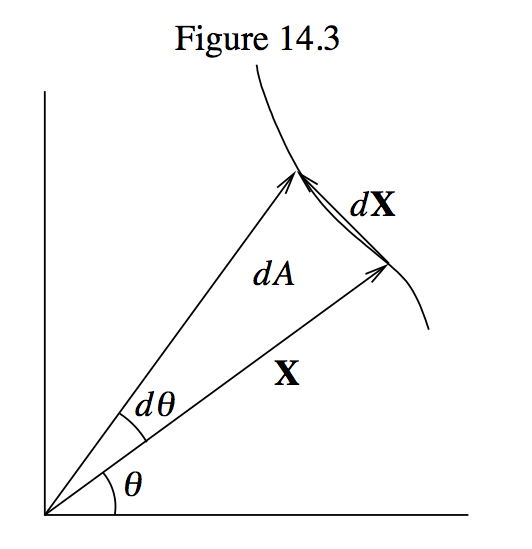
\includegraphics [scale=0.4] {Varberg14_3.png} \end{center}

As mentioned before, the problem uses $\mathbf{X}$ for the position vector, but I will label it as $\mathbf{r}$, following Feynman.  This vector "stays always in the $xy$-plane."

We are asked to show that

\[ \frac{dA}{dt} = \frac{1}{2} \ | \frac{d\mathbf{r}}{dt} \times \mathbf{r} | \]

A second change is to use dot notation

\[ \dot{\mathbf{r}} = \frac{d}{dt} \ \mathbf{r} = \mathbf{v} \]

so in looking at what is inside the brackets above, the expression is

\[ \dot{\mathbf{r}} \times \mathbf{r} \]

And if I may make an aside about this, recall that the momentum $\mathbf{p} = m \mathbf{v}$ and that the angular momentum $\mathbf{L}$ (\emph{not} the $\hat{\mathbf{L}}$ we had before) is related to what we're working with since

\[ \mathbf{L} = \mathbf{r} \times \mathbf{p} =  \mathbf{r} \times m \mathbf{v} = m(\mathbf{r} \times \mathbf{v}) =  m(\mathbf{r} \times \dot{\mathbf{r}}) =  -m(\dot{\mathbf{r}} \times \mathbf{r}) \]

And in Feynman's presentation of this which I wrote up elsewhere he shows that

\[  \frac{d}{dt} ( \mathbf{r} \times \dot{\mathbf{r}})  = \dot{\mathbf{r}} \times \dot{\mathbf{r}} +  \mathbf{r} \times  \ddot{\mathbf{r}} = 0 \]

The first term is zero because any vector's cross-product with itself is zero.  The second term is also zero by the hypothesis that the force is centripetal, toward the sun, and since, using Newton's second law that means the acceleration (which is $\ddot{\mathbf{r}}$) is also toward the sun and thus in the same direction as $-\mathbf{r}$. 

So if 

\[  \frac{d}{dt} ( \mathbf{r} \times \dot{\mathbf{r}}) = 0 \]

then let's introduce a symbol for this cross-product

\[  \mathbf{r} \times \dot{\mathbf{r}} = \mathbf{H} \]

where $\mathbf{H}$ is a constant since $d \mathbf{H}/dt = 0$ (and looking back we see that $\mathbf{L} = m \mathbf{H}$.  This is just the conservation of angular momentum.

Back to the diagram

\begin{center} 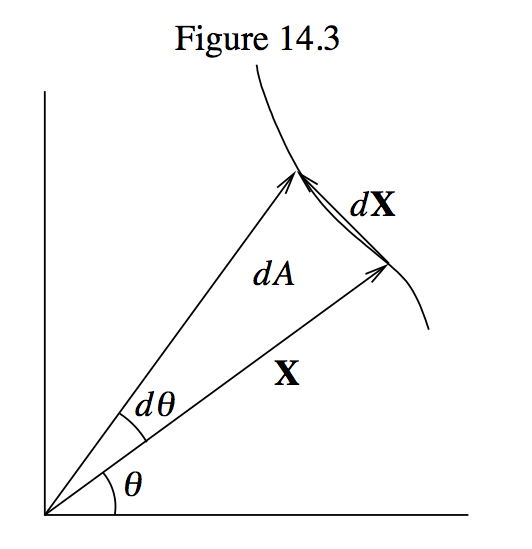
\includegraphics [scale=0.4] {Varberg14_3.png} \end{center}

In a short time, the position vector changes, and the triangle built from $\mathbf{r}(t)$ and $\mathbf{r}(t + dt)$ with third side $d\mathbf{r}$ "sweeps out" area dA.

The way we wrote it for Feynman's analysis was that the vectors were $\mathbf{r}$ and $\dot{\mathbf{r}}$ (i.e. $d\mathbf{r}/dt$).  Also, we wrote $A$ for the area of the triangle (which is $1/2 \ \mathbf{r} \times \dot{\mathbf{r}}$).

This example puzzled me because the figure has $dA$ and $d \mathbf{X}$ ($d \mathbf{r}$), whereas the statement contains the derivatives.  I think the following reasoning probably works, but I am not completely sure.

Write

\[ d\mathbf{r} = \frac{d\mathbf{r}}{dt} \ dt \]
\[ = \dot{\mathbf{r}} \ dt \]

Using the geometry and the definition of the cross-product

\[ dA = \frac{1}{2} | \mathbf{r} \times \dot{\mathbf{r}} \ dt| \]
\[ 2 \ \frac{dA}{dt} = \frac{d}{dt} \  | \mathbf{r} \times \dot{\mathbf{r}} \ dt| \]

Now differentiate the right-hand side (ignoring the vertical bars for a bit)

\[ \frac{d}{dt} \ (\mathbf{r} \times \dot{\mathbf{r}} \ dt) =  \dot{\mathbf{r}} \times \dot{\mathbf{r}} \ dt + \mathbf{r} \times \ddot{\mathbf{r}} \ dt \]

The first  term contains $\dot{\mathbf{r}} \times \dot{\mathbf{r}}$ and is clearly zero.  For the second term, in writing this, I am assuming this is legal

\[ \frac{d}{dt} \ \dot{\mathbf{r}} \ dt = \ddot{\mathbf{r}} \ dt \]

and if it is, we're good.  We have then $\ddot{\mathbf{r}} \ dt$ but that is just acceleration times the time which yields the velocity

\[ \ddot{\mathbf{r}} \ dt =  \dot{\mathbf{r}} \]

so

\[ 2 \ \frac{dA}{dt} =  | \mathbf{r} \times \dot{\mathbf{r}} | \]

which is what we were asked to prove.

Varberg \emph{et al.} give a second argument which goes as follows.  By the geometry of the triangle, the area is

\[ 2 \ dA = r \ r d \theta = r^2 d \theta \]

where $r$ is $|\mathbf{r}|$.  And then they say

\[ 2 \ \frac{dA}{dt} = r^2 \ \frac{d\theta}{dt}  \]

This result (I think) assumes that $r$ does not vary with time, but clearly it does.  The product rule would give us:

\[ \frac{d}{dt} \ r^2 d \theta = 2 r \ d \theta  \ \frac{dr}{dt} + r^2 \ \frac{d\theta}{dt}  \]

Now, perhaps you can argue that $r^2$ makes the second term much bigger, or that $dr/dt$ is very small or something.  Anyway, let's continue with the argument.

Go back to the right-hand side of what we were asked to prove above

\[ 2 \ \frac{dA}{dt} =  | \frac{d\mathbf{r}}{dt} \times \mathbf{r} | \]

and show that it turns into $r^2 d\theta/dt$.  Using $\hat{\mathbf{L}}$ for the unit vector in the $\mathbf{r}$ direction (rather than angular momentum), we have

\[ \frac{d\mathbf{r}}{dt}  = \frac{d}{dt} (r \hat{\mathbf{L}}) = \frac{dr}{dt} \hat{\mathbf{L}} + r \frac{d\hat{\mathbf{L}} }{dt}  \]

where the first part is just separating the scalar and unit vector part of $\mathbf{r}$ and the rest is from the product rule.  At this point we recall the result from the first example (that $d \hat{\mathbf{L}}/dt  = d \theta/dt \ \hat{\mathbf{L}}^{\perp}$), so we have

\[ = \frac{dr}{dt} \hat{\mathbf{L}} + r  \frac{d \theta}{dt} \ \hat{\mathbf{L}}^{\perp} \]

So now this is what we need to cross with $\mathbf{r}$, also known as $r \hat{\mathbf{L}}$.  We write

\[ (\frac{dr}{dt} \hat{\mathbf{L}} + r  \frac{d \theta}{dt} \ \hat{\mathbf{L}}^{\perp}) \times r \hat{\mathbf{L}} \]
\[ = (\frac{dr}{dt} \hat{\mathbf{L}} \times  r \hat{\mathbf{L}}) + (r  \frac{d \theta}{dt} \ \hat{\mathbf{L}}^{\perp} \times r \hat{\mathbf{L}}) \]

The first term is zero, and because these are unit vectors the absolute value of the second term's vector cross-product is $1$

\[ | r  \frac{d \theta}{dt} \ \hat{\mathbf{L}}^{\perp} \times r \hat{\mathbf{L}} | = r^2 \frac{d \theta}{dt} \]

So what we've shown is that 

\[ 2 \ \frac{dA}{dt} =  | \mathbf{r} \times \dot{\mathbf{r}} | \]

and

\[ 2 \ \frac{dA}{dt} =  r^2 \ \frac{d \theta}{dt} \]

\subsection*{Kepler's Second Law K2}

K2 says that orbits "sweep out equal areas in equal times" or equivalently, that $dA/dt = 0$.  So we start from Newton's force directed toward the sun, the centripetal force, and we will show that the motion stays in a plane, and also implies K2.

Again, this is Feynman's argument (and notation)

\[ \frac{d}{dt} ( \mathbf{r} \times \mathbf{v}) = \frac{d}{dt} ( \mathbf{r} \times \dot{\mathbf{r}}) = 0 \]

This is zero because you get two terms from the derivative of the cross-product:  one is $\dot{\mathbf{r}} \times \dot{\mathbf{r}} = 0$ , and the second one is $\mathbf{r} \times \ddot{\mathbf{r}}$, which is zero because these two vectors point in opposite directions by the centripetal force postulate.

Therefore,  $\mathbf{r} \times \dot{\mathbf{r}}$ is constant.  We will say that

\[ \mathbf{r} \times \dot{\mathbf{r}} = \mathbf{H} \]

and 

\[ |\mathbf{H}| = h = 2 \ \frac{dA}{dt} \]

If $\mathbf{H} = 0$, there is no force, and just straight-line motion.  But for  $\mathbf{H} \ne 0$, then $\mathbf{r}$ and $\dot{\mathbf{r}}$ are in a plane that doesn't change with time, and $\mathbf{H}$ is the normal vector of that plane.

\[ h = | \mathbf{r} \times \dot{\mathbf{r}} | = |\mathbf{r} \times \frac{d\mathbf{r}}{dt} | \]

by the example above ($14.5$)

\[ h =  r^2 \ \frac{d \theta}{dt} = 2 \ \frac{dA}{dt} \]

And this is K2.  $dA/dt$ is constant, equal to $h/2$.

\subsection*{reverse}

Now we are going to reverse the argument and show that planar motion and K2 imply a centripetal force.  Planar motion means that $\mathbf{r} \times \dot{\mathbf{r}}$ has fixed direction (again, normal to the plane), and K2 means that it has constant magnitude.  Since it doesn't change with time

\[ \frac{d}{dt} (\mathbf{r} \times \dot{\mathbf{r}}) = 0 \]

but 

\[ \frac{d}{dt} (\mathbf{r} \times \dot{\mathbf{r}}) = \dot{\mathbf{r}} \times \dot{\mathbf{r}} + \mathbf{r} \times \ddot{\mathbf{r}}  \]

Now $\dot{\mathbf{r}} \times \dot{\mathbf{r}}$ is always zero, so that means the second term

\[ \mathbf{r} \times \ddot{\mathbf{r}} = \mathbf{r} \times \mathbf{a} = 0 \]

The acceleration vector $\mathbf{a}$ is parallel to the position vector.

\subsection*{Kepler's First Law K1}

We make an additional hypothesis due to Newton, which is that the acceleration is proportional to the inverse square of the distance from the sun (origin), and pointed toward it.

\[ \mathbf{a} = \ddot{\mathbf{r}} = - \frac{k}{r^2} \hat{\mathbf{L}} \]

where $\hat{\mathbf{L}}$ is the \emph{unit} vector in the $\mathbf{r}$ direction (i.e. equal to $\mathbf{r}/|\mathbf{r}|$), and $k$ is a constant (namely $GM$), not to be confused with the unit vector $\hat{\mathbf{k}}$.

The first of three main steps in the proof is to take the cross-product with $\hat{\mathbf{k}}$ (as the text says, "this allows us to introduce the area information in vectorial form")

\[ \ddot{\mathbf{r}} \times \hat{\mathbf{k}} = - \frac{k}{r^2} \ \hat{\mathbf{L}} \times \hat{\mathbf{k}} = \frac{k}{r^2} \ \hat{\mathbf{L}}^{\perp} \]

(recall that we "go to the left" for $\hat{\mathbf{L}}^{\perp}$).  By example 14.4 above

\[ \frac{d\hat{\mathbf{L}}}{dt}= \frac{d\theta}{dt} \ \hat{\mathbf{L}}^{\perp} \]
\[ \hat{\mathbf{L}}^{\perp} = \frac{d \hat{\mathbf{L}}/dt}{d\theta/dt } \]

and from K2

\[ \frac{d \theta}{dt} = \frac{h}{r^2} \]

Hence

\[  \hat{\mathbf{L}}^{\perp} = \frac{d \hat{\mathbf{L}}/dt}{d \theta / dt} = \frac{d \hat{\mathbf{L}}/dt}{h/r^2} \]

So the cross-product

\[ \ddot{\mathbf{r}} \times \hat{\mathbf{k}} = \frac{k}{r^2} \ \hat{\mathbf{L}}^{\perp} = \frac{k}{h} \ \frac{d\hat{\mathbf{L}}}{dt}  \]

Now the second clever thing we do here is to integrate with respect to time (remember that $k$, $h$ and $\hat{\mathbf{k}}$ are all constant)

\[ \dot{\mathbf{r}} \times \hat{\mathbf{k}} = \frac{k}{h} \ (\hat{\mathbf{L}} + \mathbf{E}) \]

where $ \mathbf{E}$ is a constant (vector) of integration.

The third step is to dot both sides with $\mathbf{r}$

\[ \mathbf{r} \cdot ( \dot{\mathbf{r}} \times \hat{\mathbf{k}}) = \frac{k}{h} \ \mathbf{r} \cdot (\hat{\mathbf{L}} + \mathbf{E}) \]

using the following vector identity, the left-hand side is

\[ \mathbf{r} \cdot ( \dot{\mathbf{r}} \times \hat{\mathbf{k}}) = (\mathbf{r} \times \dot{\mathbf{r}}) \cdot \hat{\mathbf{k}} \]

but 

\[ \mathbf{r} \times \dot{\mathbf{r}} = h \ \hat{\mathbf{k}} \]

so we have

\[ h \ \hat{\mathbf{k}} \cdot \hat{\mathbf{k}} = h \]

Putting it all together

\[ \mathbf{r} \cdot (\ddot{\mathbf{r}} \times \hat{\mathbf{k}}) = h = \frac{k}{h} \ \mathbf{r} \cdot (\hat{\mathbf{L}} + \mathbf{E}) \]

\[ \frac{h^2}{k} =  \mathbf{r} \cdot (\hat{\mathbf{L}}+ \mathbf{E}) \]

Recall that $\hat{\mathbf{L}}$ is the unit vector in the same direction as $\mathbf{r}$ so that $\mathbf{r} \cdot \hat{\mathbf{L}} = r$.

We can take $\mathbf{E}$ to be in the direction of $\mathbf{r}$ at time-zero so $\mathbf{r} \cdot \mathbf{E}$ is equal to $r$ times $e$ times the cosine of the angle between them at some later time.  (Since $\mathbf{E}$ is a constant vector of integration, its magnitude $e$ can be anything we want).

Thus, in polar coordinates this becomes 

\[ r(1 + e \cos \theta) = \frac{h^2}{k} \]

These curves are conic sections.  If $e < 1$ it's an ellipse.

\begin{center} 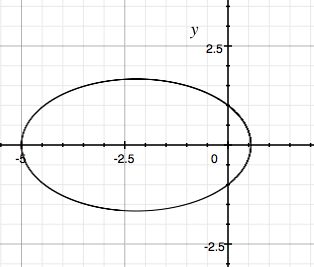
\includegraphics [scale=0.6] {quick_ellipse.png} \end{center}

The outer curve above is an ellipse with the formula

\[ r(1 + 0.1 \cos \theta) = 2 \]

(the inner is just a circle in the template that I couldn't get rid of).

$e$ is the eccentricity of the ellipse

\[ e^2 +  \frac{b^2}{a^2} = 1 \]

\subsection*{Kepler's Third Law K3}

To prove:

\[ T^2 = \frac{(2 \pi)^2}{k} \ a^3 \]

where $T$ is the period, $k$ is our constant from before, and $a$ is the length of the half-major axis of the ellipse.  In other words, the period of an orbit is the $3/2$ power of the "radius", technically the semi-major axis of the ellipse.

Start with K2

\[ 2 \ \frac{dA}{dt} =  h \]

Integrate with respect to time over one revolution obtaining an ellipse with area $\pi a b$ and the period $T$ for the time

\[ 2 \pi a b = hT \]
\[ T^2 = (\frac{2 \pi a b}{h})^2 \]

Now, go back to the equation for the orbit

\[ r(1 + e \cos \theta) = \frac{h^2}{k} \]

Consider one-half an orbit between $\theta = 0 \rightarrow \theta = \pi$.  The length of the axis is $2a$, equal to $2r$ for this orbit, so

\[ 2a = \frac{h^2}{k(1 + e \cos \pi)} +  \frac{h^2}{k(1 + e \cos 0)} \]
\[ = \frac{h^2}{k} (\frac{1}{1 - e} +  \frac{1}{1 + e}) \]
\[ = \frac{h^2}{k} \ \frac{2}{1 - e^2} \]

So

\[ a = \frac{h^2}{k} \ \frac{1}{1 - e^2} \]

For an ellipse

\[ \frac{b^2}{a^2} = 1 - e^2 \]

so
\[ a = \frac{h^2}{k} \ \frac{a^2}{b^2} \]

\[  b^2 = \frac{ah^2}{k}  \]

We had 

\[ T^2 = (\frac{2 \pi a b}{h})^2 \]
\[ = (\frac{2 \pi a }{h})^2 \  \frac{ah^2}{k}  \]
\[ = \frac{(2 \pi)^2}{k} a^3 \]

which is K3.  Recall that $k$ is $GM$, the gravitational constant times the mass of the sun.  The angular momentum $h$ has dropped out.  In other words, the period for a particular orbit does not depend on the mass of the planet or satellite.

\end{document}  